\documentclass{article}
\usepackage{fancyhdr}
\usepackage{xeCJK}
\usepackage[top=2cm, bottom=2cm, left=2cm, right=2cm]{geometry}
\usepackage{algorithm}
\usepackage{algorithmicx}
\usepackage{algpseudocode}
\usepackage{amsmath}
\usepackage{graphicx}
\usepackage{float}
\usepackage{indentfirst}
\usepackage{cite}

\setlength{\parindent}{2em}
\setCJKmainfont[BoldFont=SimHei,ItalicFont={[stkaiti.ttf]}]{SimSun}

\title{\textbf{Project Stereo}}
\author{Author:Yongshun Zhang}


\begin{document}

\maketitle
\section{Camera Basics}
\subsection{the Intrinsics and the Extrinsics of a Camera and the Camera Matrix}
\paragraph{}A \textbf{Camera Matrix} is used to denote a projective mapping from World Coordinates to Pixel Coordinates, which can be represented as follows.\cite{CameraResectioning}
\\
\begin{equation}
\emph{Camera Matirx}\ \ \mathbf{P}= K \times \left[\begin{array}{cc}R & T \end{array}
\right]
\end{equation}
In equation (1), the matrix \textbf{K} is called intrisic parameters, and the matrix [R T] is the extrinsic parameters.

\paragraph{} The intrinsic matrix \textbf{K} contains 5 intrinsic, and has the following form.
\begin{equation}
\mathbf{K}= \left[\begin{array}{cccc}
\alpha_x & \gamma & \mu_0 & 0\\
0 & \alpha_y & \upsilon_0 & 0\\
0 & 0 & 1 & 0
\end{array}
\right]
\end{equation}
These parameters encompass focal length, image sensor format and principal point(image centre). Before introducing the intrinsic matrix ,we need to know how the pixel skew is define, which is shown in Figure 1\cite{Intrinsic}.
\begin{figure}[H]
\centering
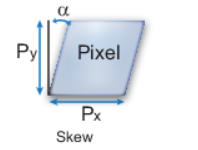
\includegraphics[scale=0.5]{1.png}
\caption{skew}
\label{fig:label}
\end{figure}
The meanings and metrics of the parameters $\alpha_x,\ \alpha_y,\ \gamma,\ \mu_0,\ \upsilon_0$ are described in tabulation 1\cite{CameraResectioning}\cite{Intrinsic}.
\\
\begin{table}[H]
\centering
\begin{tabular}{|l|}
\hline
\\
$(\mu_0,\ \upsilon_0)$ // Principal point, in pixels\\
\\
\hline
\\
$(\alpha_x,\ \alpha_y)$ //focal length, in pixels\\
\\
$\alpha_x \ \gets F / p_x$, $\alpha_y \ \gets F / p_y$
F // Focal length in world units, typically expressed in millimeters\\
\\
$(p_x,\ p_y)$  //  Size of the pixel in world units \\
\\
\hline
\\
s $\gets \ alpha_y * tan(\alpha)$  //  Skew coefficient\\
\\
\hline
\end{tabular}
\caption{parameters of intrinsic matrix}
\label{tab:label}
\end{table}
\paragraph{} Extrinsic parameters consisting of matrix \textbf{R},\textbf{T}, are the extrinsic parameters which denote the coordinate system transformations from 3D world coordinates to 3D camera coordinates. Extrinsic parameters define the position of camera center and the camera's heading in real world. \textbf{T} is the position of the origin of the world coordinate system expressed in coordinates of camera-centered coordinate system, \textbf{R} is a rotation matrix used to perform a rotation in Euclidean space, which properties are $\mathbf{R}^T = \mathbf{R}^{-1}$ and det \textbf{R}=1 \cite{RotationMatrix}.
\paragraph{} Often, we use $[\mu\ \upsilon\ 1]^T$ to represent a 2D point position in pixel coordinates, and $[x_w\ y_w\ z_w\ 1]^T$ is used to present a 3D point position in world coordinates, which are expressed in augmented notation of Homogeneous coordinates. Referring to the pinhole camera model, the camera matrix denotes a projective mapping from world coordinates to pixel coordinates.
\begin{equation}
z^c \times \left[\begin{array}{c}
\mu\\
\upsilon\\
1
\end{array}
\right] = K \times \left[\begin{array}{cc}R & T \end{array}\right] \times \left[\begin{array}{c}
x_w\\
y_w\\
z_w\\
1
\end{array}
\right]
\end{equation}
$z_c$ represents the coordinate of z axis in used to make the constant of proportionality of two matrices\cite{ScaleFactor}.
\paragraph{Problems} There are some little problems during learning Camera Matrix. The first is the position, \textbf{C}, of the camera expressed in world coordinate, I didn't understand the equation $\mathbf{C}\ =\ -\mathbf{R}_{-1}\mathbf{T}\ =\ -\mathbf{R}_T\mathbf{T}$ originally, and I find the answer in the meaning of the Homogeneous coordinates. When we transfer the coordinates from 3D world to 2D pixel, the coordinate expressed in Homogeneous coordinates can realize rotation, zoom and translation, so translation T, which represents the origin of world coordinates expressed in pixel coordinates, used to make the 2D pixel coordinate taking the origin of pixel coordinates(image centre) as its origin of coordinates. And the second problem is that the five intrinsic parameters in matrix \textbf{K} are expressed indistinct in wikipedia, and I found the distinct expression in MathWorks website\cite{Intrinsic}, which is shown in tabulation 1.
\paragraph{Written by Yongshun, 22:00, 21th Mar 2018}

\subsection{Camera Imaging}
\paragraph{Problems}When I start to deal with the transform question, I find that I'm still in a preliminary understanding of camera resectioning and camera matrix, so I read the detailed introduction of \textbf{Camera Matrix}\cite{CameraMatrix} and the \textbf{Pinhole Camera model}\cite{Pinhole} from wikipedia firstly, and have a progressive understanding of Camera Matrix including its relation with pinhole camera model and the derivation of its equation. But the next problem comes, I find that I'm confused of the axes' directions and the relationship between principal point's coordinate and optical centre's coordinate.
\paragraph{}So I try to search the relationship between principal point and optical centre by Google, such as "the relationship between principal point and optical centre" and also try to search in Chinese, finally I found the relationship between in wikipedia "Pinhole Camera Model"\cite{Pinhole}, it tells "A point R at the intersection of the optical axis and the image plane. This point is referred to as the principal point or image center.". As for the axes' directions, I review the web pages about the camera matrix, camera resectioning I have read, and also read some documents and blogs\cite{COMP}\cite{csdn1}\cite{zhopencv}, and finally solve the problem temporarily.
\paragraph{}The answer of transform is as follows.
\\
\paragraph{}First, transform the 3D point \textbf{X} from World coordinates to Camera coordinates, using the extrinsic parameters.$[X_c,\ Y_c,\ Z_c]_T$ represents the point in Camera coordinates.
\\
\begin{equation}
\left[\begin{array}{c}
X_c\\
Y_c\\
Z_c
\end{array}
\right] = \left[\begin{array}{cc}
R & T
\end{array}
\right] \times \left[\begin{array}{c}
X_1\\
X_2\\
X_3\\
1
\end{array}
\right]
\end{equation}
\\
\paragraph{}Second, transform the 3D point in Camera coordinates to 2D point in Image plane.
\\
\begin{equation}
Z_c \times \left[\begin{array}{c}
x\\
y\\
1
\end{array}
\right] =  \left[\begin{array}{ccc}
f_x & 0 & 0\\
0 & f_y & 0\\
0 & 0 & 1
\end{array}
\right] \times \left[\begin{array}{c}
X_c\\
Y_c\\
Z_c\\
\end{array}
\right]
\end{equation}
\\
\paragraph{}Finally, transform the 2D point from image plane to pixel coordinates.
\\
\begin{equation}
u = x + c_x,\ \ v = y + c_y
\end{equation}
\\
\paragraph{}All equations above can be replaced with the following one.
\begin{equation}
Z_c \times \left[\begin{array}{c}
\mu\\
\upsilon\\
1
\end{array}
\right] = \left[\begin{array}{ccc}
f_x & 0 & c_x\\
0 & f_y & c_y\\
0 & 0 & 1
\end{array}
\right] \times \left[\begin{array}{cc}R & t \end{array}\right] \times \left[\begin{array}{c}
X_1\\
X_2\\
X_3\\
1
\end{array}
\right]
\end{equation}
\\
\subsection{Relationship Between 2D Image Point and 3D Camera Coordinate}
\paragraph{}A 2D image point ($\mu,\ \upsilon$) correspond to a line in 3D camera coordinate. The derivation is as follows.
\paragraph{}\noindent First, transform the image point ($\mu,\ \upsilon$) from pixel coordinate to image plane.
\\
\begin{equation}
x = (\mu - \mu_0),\ \ \ y = (\upsilon - \upsilon_0)
\end{equation}
\\
Second, according to the pinhole camera model, transform the point from image plane to camera coordinate.
\\
\begin{equation}
X_c = x \times \frac{Z_c}{f},\ \ \ Y_c = y \times \frac{Z_c}{f}
\end{equation}
\\
According to equation (9), we set $\frac{x}{f}=k,\ \frac{y}{f}=t$, k and t are constants, so the 3D point in camera coordinate can be describe as $Z_c \times (k,\ t,\ 1)$, which represents a line in 3D coordinate.
\paragraph{Written by Yongshun, 00:43, 22th Mar 2018}

\subsection{Distortion}
\paragraph{}When I read the Camera Calibration and 3D Construction in opencv website\cite{OpencvCameraCalibration}, I find that I once read this document which has been translated in Chinese\cite{zhopencv}, and I read the document again carefully and review the introduction of distortion in Mathworks\cite{Intrinsic}.
\paragraph{}As for distortions in camera calibration, it can be classified into two types: radial distortion and tangential distortion, real lenses usually have some distortion, mostly radial distortion and slight tangential distortion.
\paragraph{}Figure 2 show two common types of Radial distortion: barrel distortion(typically $k_1>0$) and pincushion distortion(typically $k_1<0$).
\begin{figure}[H]
\centering

\includegraphics[scale=0.5]{2.png}
\caption{Radial Distortion}
\label{fig:label}
\end{figure}
\paragraph{}Tangential distortion occurs when the lens and the image plane are not parallel, shown in Figure 3.
\begin{figure}[H]
\centering

\includegraphics[scale=0.5]{3.png}
\caption{Tangential Distortion}
\label{fig:label}
\end{figure}
\paragraph{}When the distortions are considered, the camera resectioning model will be extend as:
\begin{equation}
\left[\begin{array}{c}
X_c\\
Y_c\\
Z_c
\end{array}
\right] =  \left[\begin{array}{cc}
R & T
\end{array}
\right] \times \left[\begin{array}{c}
X_w\\
Y_w\\
Z_w\\
\end{array}
\right]
\end{equation}
\begin{equation}
x = \frac{X_c}{Z_c},\ \ \ y = \frac{Y_c}{Z_c}
\end{equation}
\\
\begin{equation}
\begin{align}
x_d &= x \times \frac{1+k_1r^2+k_2r^4+k_3r^6}{1+k_4r^2+k_5r^4+k_6r^6} + 2p_1xy + p_2(r^2 + 2x^2)\\
y_d &= y \times \frac{1+k_1r^2+k_2r^4+k_3r^6}{1+k_4r^2+k_5r^4+k_6r^6} + 2p_1(r^2 + 2y^2) + 2p_2xy \\
&r^2 = x^2 + y^2
\end{align}
\end{equation}
\\
\begin{equation}
u = f_x \times x_d + c_x,\ \ v = f_y \times y_d + c_y
\end{equation}
\paragraph{Find the Origin Point} Considering the distortion model with 2 distortion coefficients, the transform equation with distortions is as follows. Point (x,y) represents the ideal point without distortion.
\begin{equation}
\begin{align}
\check{x} &= x + x(k_1(x^2+y^2)+k_2(x^2+y^2)^2)\\
\check{y} &= y + y(k_1(x^2+y^2)+k_2(x^2+y^2)^2)
\end{align}
\end{equation}
And we have
\begin{equation}
\begin{align}
\check{x} &= \frac{u - u_0}{f}\\
\check{y} &= \frac{u - u_0}{f}\\
\end{align}
\end{equation}
Then we make a square of each equation in (14), and add them together, we got
\begin{equation}
\check{x}^2 + \check{y}^2 = (x^2+y^2) + 2k_1(x^2+y^2)^2+(2k_2+k_1^2)(x^2+y^2)^3+2k_1k_2(x^2+y^2)^4+k_2^2(x^2+y^2)^5
\end{equation}
This is a liner equation of $(x^2+y^2)$, we can solve it by gradient descent. After we get the value of $(x^2+y^2)$, we get the origin point (x, y) by bring $(x^2+y^2)$ into equation (14).
\subsection{Calibration}
\paragraph{}
Base on what I know about Camera Calibration, I reckon that Camera Calibration aims to get an exact approximation of the intrinsic parameters including the distortion coefficients which only depends on the camera itself, and extrinsic parameters which represent the camera's direction and location in 3D space.
\paragraph{Written by Yongshun, 22:26, 23th Mar 2018}

\subsection{Calibration with Opencv}
\paragraph{}Before I start to use the opencv functions to calibrate the camera, I read the APIs in camera calibration introduction on OpenCV website\cite{OpencvCameraCalibration}, and sample code of camera calibration using OpenCV on github\cite{CalibrationGithub}.
\paragraph{}

\begin{thebibliography}{99}
\bibitem{CameraResectioning}\textbf{Camera resectioning}  Wikipedia  https://en.wikipedia.org/wiki/Camera\_resectioning
\bibitem{Intrinsic}\textbf{What Is Camera Calibration?}  MathWorks  https://cn.mathworks.com/help/vision/ug/camera-calibration.html?s\_tid=gn\_loc\_drop
\bibitem{RotationMatrix}\textbf{Rotation matrix}  Wikipedia   https://en.wikipedia.org/wiki/Rotation\_matrix
\bibitem{ScaleFactor}\textbf{Scale factor}  Wikipedia  https://en.wikipedia.org/wiki/Scale\_factor
\bibitem{CameraMatrix}\textbf{Camera Matrix}   Wikipedia  https://en.wikipedia.org/wiki/Camera\_matrix
\bibitem{Pinhole}\textbf{Pinhole Camera Model}   Wikipedia   https://en.wikipedia.org/wiki/Pinhole\_camera\_model
\bibitem{COMP}\textbf{Fundamentals of Computer Vision} Magill University  http://www.cim.mcgill.ca/\%7Elanger/558/4-cameramodel.pdf
\bibitem{csdn1}\textbf{关于OpenCV的那些事——相机标定}   CSDN   https://blog.csdn.net/aptx704610875/article/details/48914043
\bibitem{zhopencv}\textbf{Cv照相机标定和三维重建}   Opencv  http://wiki.opencv.org.cn/index.php/Cv\%E7\%85\%A7\%E7\%9B\%B8\%E6\%9C\%BA\%E5\%AE\%9A\%E6\%A0\%87\%E5\%92\%8C\%E4\%B8\%89\%E7\%BB\%B4\%E9\%87\%8D\%E5\%BB\%BA
\bibitem{OpencvCameraCalibration}\textbf{Camera Calibration and 3D Reconstruction} Opencv
    https://docs.opencv.org/2.4/modules/calib3d/doc/camera\_calibration\_and\_3d\_reconstruction.html
\bibitem{CalibrationGithub}\textbf{Camera Calibration and 3D Reconstruction} Opencv
    https://docs.opencv.org/2.4/modules/calib3d/doc/camera\_calibration\_and\_3d\_reconstruction.html
\end{thebibliography}

\end{document}
